\documentclass[tikz,border=12pt]{standalone}
\usetikzlibrary{arrows.meta, positioning, calc}

\tikzset{
  box/.style={
    draw,
    rounded corners=3pt,
    fill=white,
    align=center,
    font=\small,
    minimum width=4.2cm,
    minimum height=1.05cm,
    text width=4.2cm,
    inner sep=5pt
  },
  wide/.style={
    draw,
    rounded corners=3pt,
    fill=white,
    align=center,
    font=\small,
    minimum width=5.2cm,
    minimum height=1.05cm,
    text width=5.2cm,
    inner sep=5pt
  },
  input/.style={box, fill=blue!6, draw=blue!55},
  cfg/.style={box, fill=yellow!10, draw=yellow!60!black},
  env/.style={wide, fill=orange!9, draw=orange!75!black},
  comp/.style={box, fill=green!6, draw=green!45!black},
  outputbox/.style={box, fill=purple!6, draw=purple!60},
  bus/.style={wide, fill=gray!7, draw=gray!60},
  arrow/.style={-{Latex[length=2.4mm]}, thick},
  dashedarrow/.style={-{Latex[length=2.4mm]}, thick, dashed}
}

\begin{document}
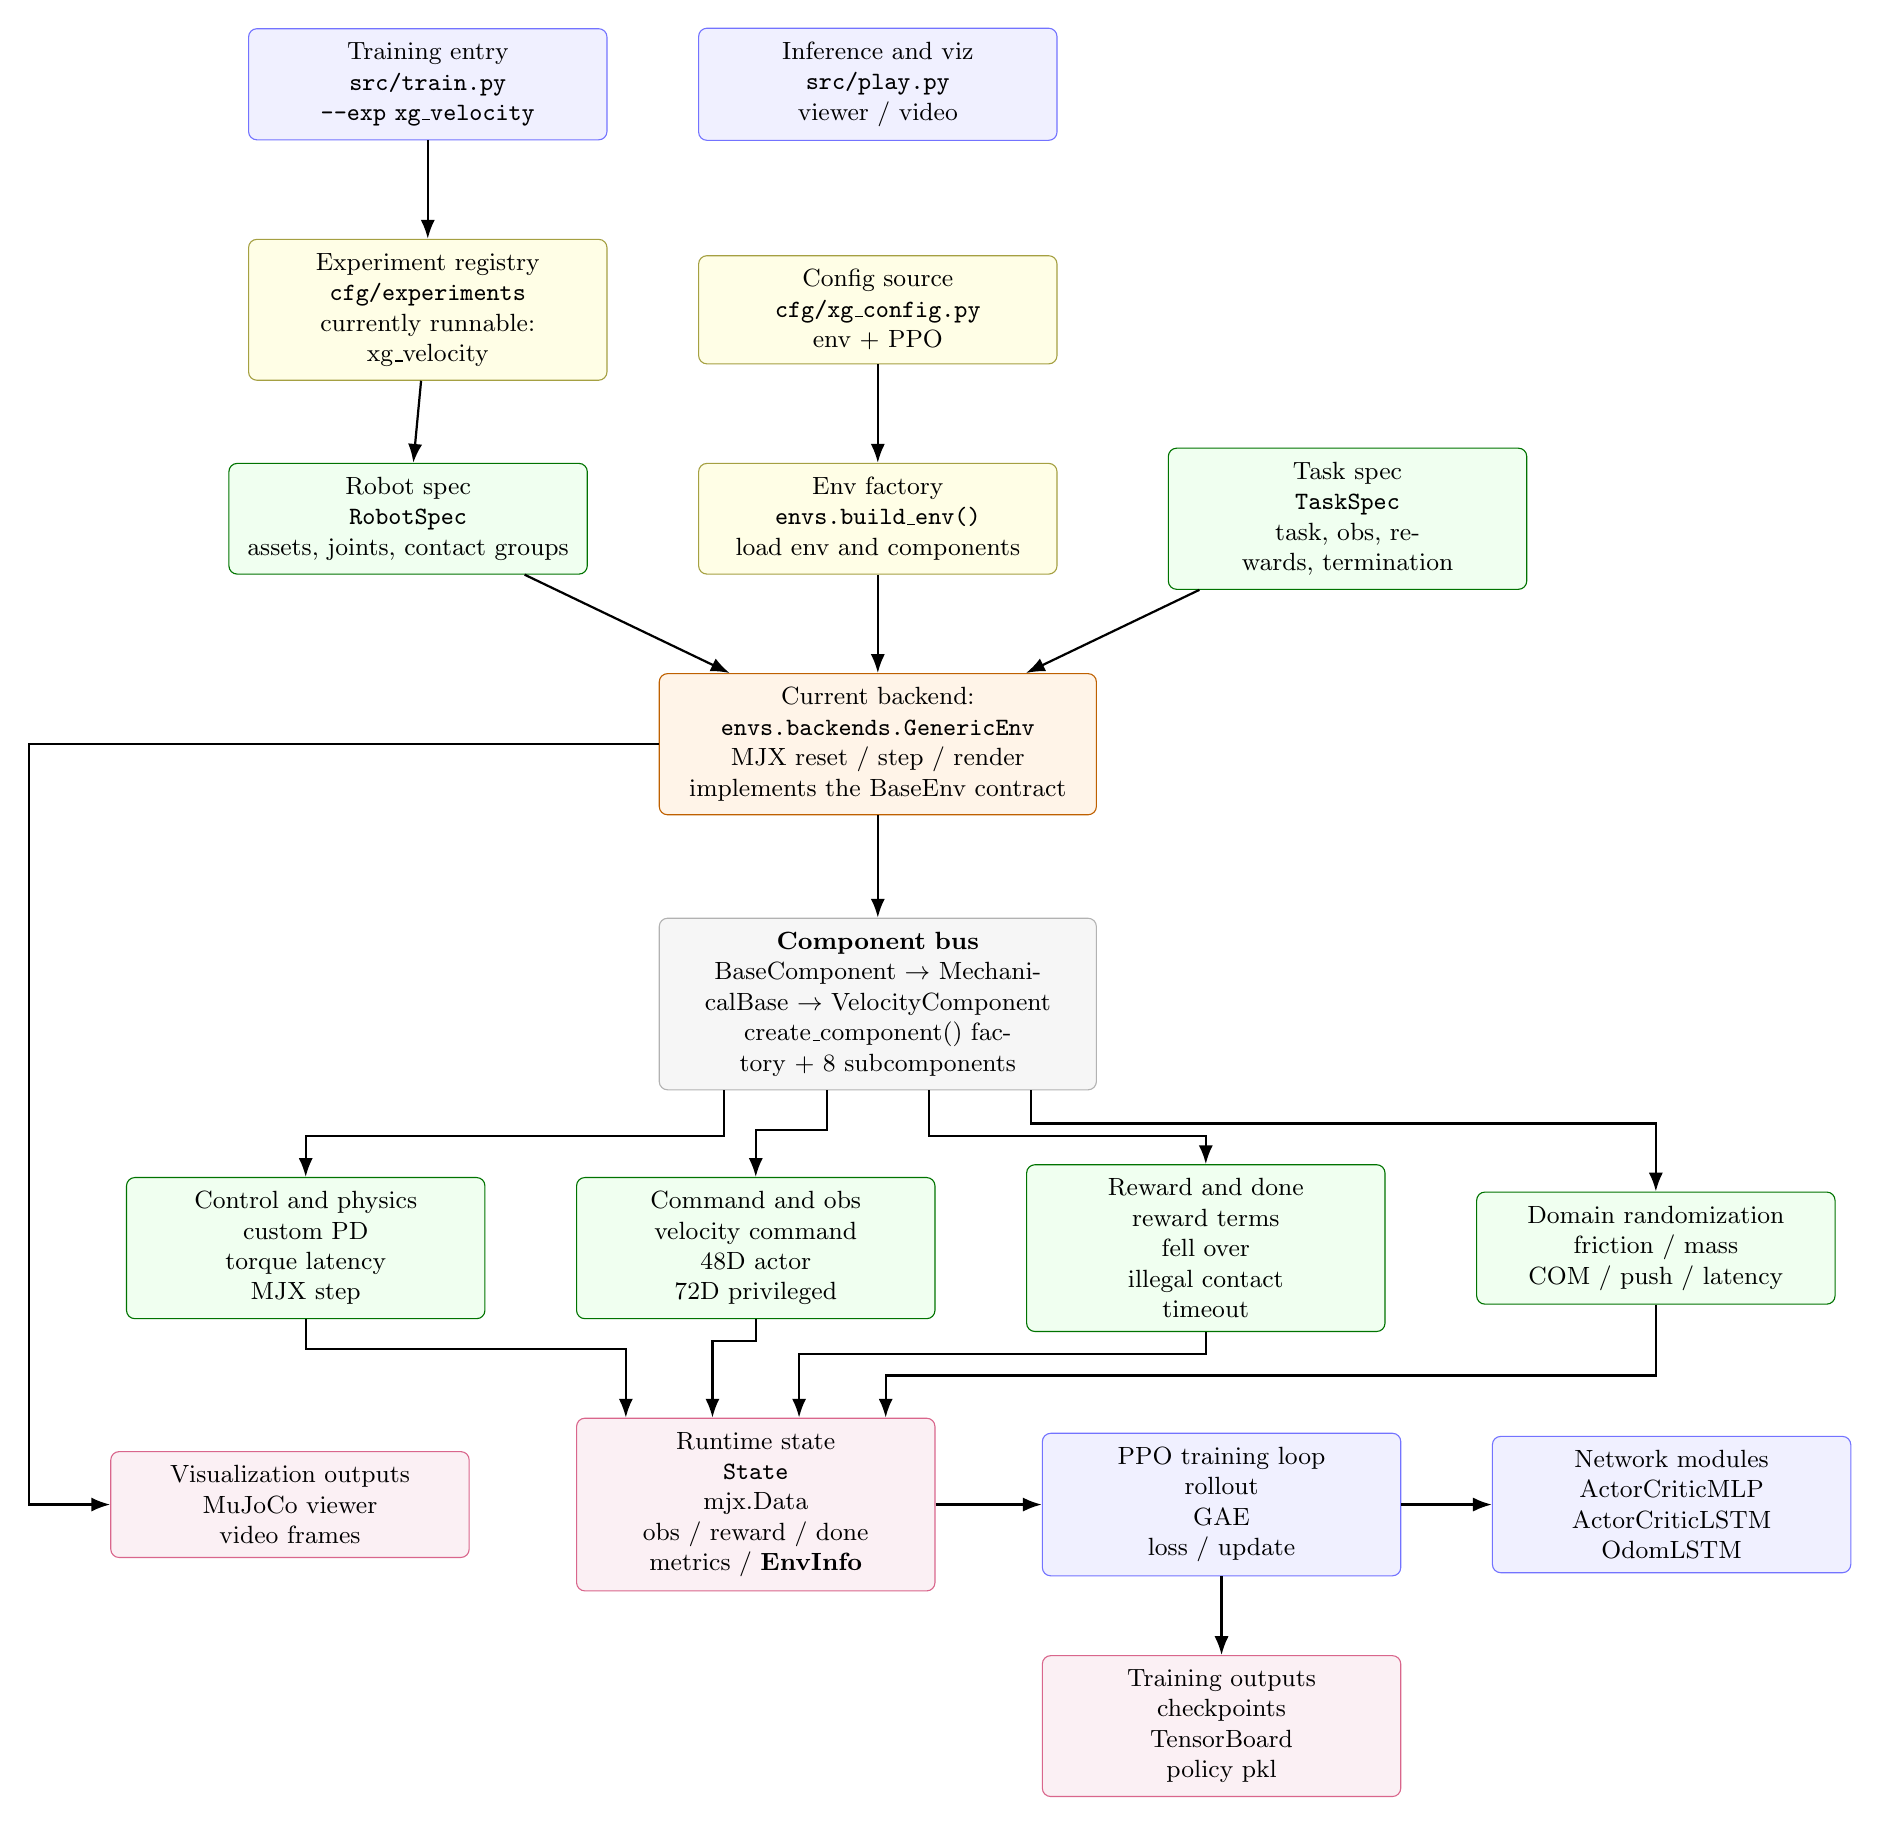
\begin{tikzpicture}[node distance=1.0cm and 1.15cm]

% Layer 1: entry points
\node[input] (TrainCLI) {Training entry\\\texttt{src/train.py}\\\texttt{--exp xg\_velocity}};
\node[input, right=of TrainCLI] (PlayCLI) {Inference and viz\\\texttt{src/play.py}\\viewer / video};

% Layer 2: experiment config
\node[cfg, below=1.25cm of TrainCLI] (Registry) {Experiment registry\\\texttt{cfg/experiments}\\currently runnable: xg\_velocity};
\node[cfg, right=of Registry] (Configs) {Config source\\\texttt{cfg/xg\_config.py}\\env + PPO};

% Layer 3: factory and specs
\node[cfg, below=1.25cm of Configs] (Factory) {Env factory\\\texttt{envs.build\_env()}\\load env and components};
\node[comp, left=1.4cm of Factory] (RobotSpec) {Robot spec\\\texttt{RobotSpec}\\assets, joints, contact groups};
\node[comp, right=1.4cm of Factory] (TaskSpec) {Task spec\\\texttt{TaskSpec}\\task, obs, rewards, termination};

% Layer 4: backend
\node[env, below=1.25cm of Factory] (Env) {Current backend: \texttt{envs.backends.GenericEnv}\\MJX reset / step / render\\implements the BaseEnv contract};

\node[bus, below=1.3cm of Env] (ComponentBus) {
  \textbf{Component bus}\\
  BaseComponent $\to$ MechanicalBase $\to$ VelocityComponent\\
  create\_component() factory + 8 subcomponents
};

% Layer 6: split detailed components below bus.
\node[comp, below left=1.1cm and 2.2cm of ComponentBus] (Control) {Control and physics\\custom PD\\torque latency\\MJX step};
\node[comp, right=of Control] (ObsCmd) {Command and obs\\velocity command\\48D actor\\72D privileged};
\node[comp, right=of ObsCmd] (RewardDone) {Reward and done\\reward terms\\fell over\\illegal contact\\timeout};
\node[comp, right=of RewardDone] (DomainRand) {Domain randomization\\friction / mass\\COM / push / latency};

% Layer 7: state, training, outputs
\node[outputbox, below=1.25cm of ObsCmd] (State) {Runtime state\\\texttt{State}\\mjx.Data\\obs / reward / done\\metrics / \textbf{EnvInfo}};
\node[input, right=1.35cm of State] (PPO) {PPO training loop\\rollout\\GAE\\loss / update};
\node[input, right=of PPO] (Networks) {Network modules\\ActorCriticMLP\\ActorCriticLSTM\\OdomLSTM};
\node[outputbox, below=of PPO] (Checkpoints) {Training outputs\\checkpoints\\TensorBoard\\policy pkl};
\node[outputbox, left=1.35cm of State] (Viewer) {Visualization outputs\\MuJoCo viewer\\video frames};

% Clean main flow, only adjacent layers.
\draw[arrow] (TrainCLI) -- (Registry);
\draw[arrow] (Registry) -- (RobotSpec);
\draw[arrow] (Configs) -- (Factory);
\draw[arrow] (RobotSpec) -- (Env);
\draw[arrow] (Factory) -- (Env);
\draw[arrow] (TaskSpec) -- (Env);
\draw[arrow] (Env) -- (ComponentBus);

\draw[arrow] ([xshift=-1.95cm]ComponentBus.south) -- ++(0,-0.58) -| (Control.north);
\draw[arrow] ([xshift=-0.65cm]ComponentBus.south) -- ++(0,-0.50) -| (ObsCmd.north);
\draw[arrow] ([xshift=0.65cm]ComponentBus.south) -- ++(0,-0.58) -| (RewardDone.north);
\draw[arrow] ([xshift=1.95cm]ComponentBus.south) -- ++(0,-0.42) -| (DomainRand.north);

\draw[arrow] (Control.south) -- ++(0,-0.38) -| ([xshift=-1.65cm]State.north);
\draw[arrow] (ObsCmd.south) -- ++(0,-0.28) -| ([xshift=-0.55cm]State.north);
\draw[arrow] (RewardDone.south) -- ++(0,-0.28) -| ([xshift=0.55cm]State.north);
\draw[arrow] (DomainRand.south) -- ++(0,-0.9) -| ([xshift=1.65cm]State.north);

\draw[arrow] (State) -- (PPO);
\draw[arrow] (PPO) -- (Networks);
\draw[arrow] (PPO) -- (Checkpoints);
\draw[arrow] (Env.west) -- ++(-8.0,0) |- (Viewer.west);

\end{tikzpicture}
\end{document}
